\documentclass[oneside,11pt,a4paper]{article}

% PACKAGES %

\usepackage[utf8]{inputenc}    
\usepackage[T1]{fontenc}
\usepackage[francais]{babel}
\usepackage{graphicx}
\usepackage{layout}
\usepackage{color}
\usepackage{lipsum}
\usepackage{tikz}
\usepackage{lscape}
\usepackage{listings}
\usepackage{amsmath}
\usepackage{amssymb}
\usepackage{placeins}
\usepackage{array}
%\usepackage[active,tightpage]{preview}

% D�fini les marges � 2 cm
\usepackage[top=1cm, bottom=2cm, left=2.5cm, right=2.5cm]{geometry}

% Supprime l'indentation de la premi�re ligne des paragraphes
\setlength{\parindent}{0pt}
\setlength{\parskip}{10pt}

\definecolor{keywordsColor}{rgb}{0,0.5,0}

\lstset{ %
  backgroundcolor=\color{white},   % choose the background color; you must add \usepackage{color} or \usepackage{xcolor}
  basicstyle=\footnotesize\ttfamily,        % the size of the fonts that are used for the code
  breakatwhitespace=false,         % sets if automatic breaks should only happen at whitespace
  breaklines=true,                 % sets automatic line breaking
  captionpos=none,                    % sets the caption-position to none
  columns=fixed,
  commentstyle=\color{green},    % comment style
  escapeinside={\%*}{*)},          % if you want to add LaTeX within your code
  extendedchars=true,              % lets you use non-ASCII characters; for 8-bits encodings only, does not work with UTF-8
 % frame=single,                    % adds a frame around the code
  keywordstyle=\bfseries\color{keywordsColor},       % keyword style
  language=SQL,                 % the language of the code
  numbers=left,                    % where to put the line-numbers; possible values are (none, left, right)
  numbersep=10pt,                   % how far the line-numbers are from the code
  numberstyle=\tiny\color{gray}, % the style that is used for the line-numbers
  morekeywords={REFERENCES},
  deletekeywords={YEAR},
  rulecolor=\color{black},         % if not set, the frame-color may be changed on line-breaks within not-black text (e.g. comments (green here))
  showspaces=false,                % show spaces everywhere adding particular underscores; it overrides 'showstringspaces'
  showstringspaces=false,          % underline spaces within strings only
  showtabs=false,                  % show tabs within strings adding particular underscores
  stepnumber=1,                    % the step between two line-numbers. If it's 1, each line will be numbered
  stringstyle=\color{blue},     % string literal style
  tabsize=2,                       % sets default tabsize to 2 spaces
  title=\lstname                   % show the filename of files included with \lstinputlisting; also try caption instead of title
}

% DOCUMENT %

\begin{document}
\title{Database project - deliverable 1}
\author{
	Arthur \bsc{Giroux}\\\small{205443}
	\and
	Colla \bsc{Rensch}\\\small{205814}
	\and
	Valentin \bsc{Matter}\\\small{203447}
}
\date{March $^{24th}$ 2013} 

\maketitle

\section{ER model}

\begin{center}
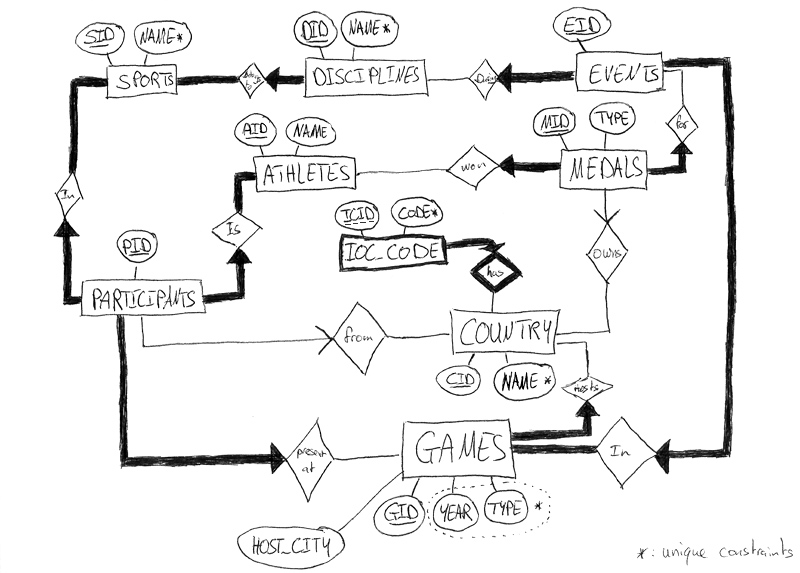
\includegraphics[height=310px]{ermodel.jpg}
\end{center}

\noindent\hrulefill

\section{Tables creation}

\lstinputlisting{db.sql}

\noindent\hrulefill

\section{Remarks}

\begin{itemize}
	\item Athletes is the entity that stores the information of an athlete who can then participate in multiple sports or games. Which means that if an Athele competes twice he will have only one entry in the ATHLETE table but two in the PARTICIPANTS table.
	\item Each game should at least have one event otherwise soothing happened during he games. The same applies to sports, a sport must have at least one participant, other wise the sport never took place during any games.
	\item Countries, sports and disciplines must have a unique name as the opposite would have no sense. For games it is the pair YEAR,TYPE that must be unique.
	\item Due to problem with their federations some athletes may present themselves without representing a country.
	\item Some medals could not be associated to a country as some athletes aren't as for the above point.
	\item The numbers of countries, athletes and events for a given game isn't stored in the GAMES entity as they can be easily computed.
\end{itemize}

\noindent\hrulefill

\end{document}